%% bare_jrnl.tex
%% V1.4b
%% 2015/08/26
%% by Michael Shell
%% see http://www.michaelshell.org/
%% for current contact information.
%%
%% This is a skeleton file demonstrating the use of IEEEtran.cls
%% (requires IEEEtran.cls version 1.8b or later) with an IEEE
%% journal paper.
%%
%% Support sites:
%% http://www.michaelshell.org/tex/ieeetran/
%% http://www.ctan.org/pkg/ieeetran
%% and
%% http://www.ieee.org/

%%*************************************************************************
%% Legal Notice:
%% This code is offered as-is without any warranty either expressed or
%% implied; without even the implied warranty of MERCHANTABILITY or
%% FITNESS FOR A PARTICULAR PURPOSE! 
%% User assumes all risk.
%% In no event shall the IEEE or any contributor to this code be liable for
%% any damages or losses, including, but not limited to, incidental,
%% consequential, or any other damages, resulting from the use or misuse
%% of any information contained here.
%%
%% All comments are the opinions of their respective authors and are not
%% necessarily endorsed by the IEEE.
%%
%% This work is distributed under the LaTeX Project Public License (LPPL)
%% ( http://www.latex-project.org/ ) version 1.3, and may be freely used,
%% distributed and modified. A copy of the LPPL, version 1.3, is included
%% in the base LaTeX documentation of all distributions of LaTeX released
%% 2003/12/01 or later.
%% Retain all contribution notices and credits.
%% ** Modified files should be clearly indicated as such, including  **
%% ** renaming them and changing author support contact information. **
%%*************************************************************************


% *** Authors should verify (and, if needed, correct) their LaTeX system  ***
% *** with the testflow diagnostic prior to trusting their LaTeX platform ***
% *** with production work. The IEEE's font choices and paper sizes can   ***
% *** trigger bugs that do not appear when using other class files.       ***                          ***
% The testflow support page is at:
% http://www.michaelshell.org/tex/testflow/



% \documentclass[journal, english]{IEEEtran} %
\documentclass[onecolumn, journal, english, 12pt, a4paper]{IEEEtran} %
% \documentclass[12pt]{article}


%
% If IEEEtran.cls has not been installed into the LaTeX system files,
% manually specify the path to it like:
% \documentclass[journal]{../sty/IEEEtran}





% Some very useful LaTeX packages include:
% (uncomment the ones you want to load)


% *** MISC UTILITY PACKAGES ***
%
%\usepackage{ifpdf}
% Heiko Oberdiek's ifpdf.sty is very useful if you need conditional
% compilation based on whether the output is pdf or dvi.
% usage:
% \ifpdf
%   % pdf code
% \else
%   % dvi code
% \fi
% The latest version of ifpdf.sty can be obtained from:
% http://www.ctan.org/pkg/ifpdf
% Also, note that IEEEtran.cls V1.7 and later provides a builtin
% \ifCLASSINFOpdf conditional that works the same way.
% When switching from latex to pdflatex and vice-versa, the compiler may
% have to be run twice to clear warning/error messages.






% *** CITATION PACKAGES ***
%
% \usepackage{cite}
% cite.sty was written by Donald Arseneau
% V1.6 and later of IEEEtran pre-defines the format of the cite.sty package
% \cite{} output to follow that of the IEEE. Loading the cite package will
% result in citation numbers being automatically sorted and properly
% "compressed/ranged". e.g., [1], [9], [2], [7], [5], [6] without using
% cite.sty will become [1], [2], [5]--[7], [9] using cite.sty. cite.sty's
% \cite will automatically add leading space, if needed. Use cite.sty's
% noadjust option (cite.sty V3.8 and later) if you want to turn this off
% such as if a citation ever needs to be enclosed in parenthesis.
% cite.sty is already installed on most LaTeX systems. Be sure and use
% version 5.0 (2009-03-20) and later if using hyperref.sty.
% The latest version can be obtained at:
% http://www.ctan.org/pkg/cite
% The documentation is contained in the cite.sty file itself.

\usepackage[utf8]{inputenc}
% \usepackage[spanish]{babel}
\usepackage{babel,csquotes,xpatch}  % recommended
% \usepackage[backend=biber,style=ieee]{biblatex}
\usepackage[backend=biber, style=ieee, maxnames=9]{biblatex}
\addbibresource{./bibtex/bib/bibliography.bib}





% *** GRAPHICS RELATED PACKAGES ***
%
\ifCLASSINFOpdf
   \usepackage[pdftex]{graphicx}
  % declare the path(s) where your graphic files are
  % \graphicspath{{../pdf/}{../jpeg/}}
  % and their extensions so you won't have to specify these with
  % every instance of \includegraphics
  % \DeclareGraphicsExtensions{.pdf,.jpeg,.png}
\else
  % or other class option (dvipsone, dvipdf, if not using dvips). graphicx
  % will default to the driver specified in the system graphics.cfg if no
  % driver is specified.
  % \usepackage[dvips]{graphicx}
  % declare the path(s) where your graphic files are
  % \graphicspath{{../eps/}}
  % and their extensions so you won't have to specify these with
  % every instance of \includegraphics
  % \DeclareGraphicsExtensions{.eps}
\fi
% graphicx was written by David Carlisle and Sebastian Rahtz. It is
% required if you want graphics, photos, etc. graphicx.sty is already
% installed on most LaTeX systems. The latest version and documentation
% can be obtained at: 
% http://www.ctan.org/pkg/graphicx
% Another good source of documentation is "Using Imported Graphics in
% LaTeX2e" by Keith Reckdahl which can be found at:
% http://www.ctan.org/pkg/epslatex
%
% latex, and pdflatex in dvi mode, support graphics in encapsulated
% postscript (.eps) format. pdflatex in pdf mode supports graphics
% in .pdf, .jpeg, .png and .mps (metapost) formats. Users should ensure
% that all non-photo figures use a vector format (.eps, .pdf, .mps) and
% not a bitmapped formats (.jpeg, .png). The IEEE frowns on bitmapped formats
% which can result in "jaggedy"/blurry rendering of lines and letters as
% well as large increases in file sizes.
%
% You can find documentation about the pdfTeX application at:
% http://www.tug.org/applications/pdftex





% *** MATH PACKAGES ***
%
\usepackage{amsmath, bm}
\usepackage{amssymb}
\usepackage{amsfonts}
\usepackage{mathrsfs}
\usepackage{mathtools}
% A popular package from the American Mathematical Society that provides
% many useful and powerful commands for dealing with mathematics.
%
% Note that the amsmath package sets \interdisplaylinepenalty to 10000
% thus preventing page breaks from occurring within multiline equations. Use:
%\interdisplaylinepenalty=2500
% after loading amsmath to restore such page breaks as IEEEtran.cls normally
% does. amsmath.sty is already installed on most LaTeX systems. The latest
% version and documentation can be obtained at:
% http://www.ctan.org/pkg/amsmath





% *** SPECIALIZED LIST PACKAGES ***
%
%\usepackage{algorithmic}
% algorithmic.sty was written by Peter Williams and Rogerio Brito.
% This package provides an algorithmic environment fo describing algorithms.
% You can use the algorithmic environment in-text or within a figure
% environment to provide for a floating algorithm. Do NOT use the algorithm
% floating environment provided by algorithm.sty (by the same authors) or
% algorithm2e.sty (by Christophe Fiorio) as the IEEE does not use dedicated
% algorithm float types and packages that provide these will not provide
% correct IEEE style captions. The latest version and documentation of
% algorithmic.sty can be obtained at:
% http://www.ctan.org/pkg/algorithms
% Also of interest may be the (relatively newer and more customizable)
% algorithmicx.sty package by Szasz Janos:
% http://www.ctan.org/pkg/algorithmicx




% *** ALIGNMENT PACKAGES ***
%
\usepackage{array}
% Frank Mittelbach's and David Carlisle's array.sty patches and improves
% the standard LaTeX2e array and tabular environments to provide better
% appearance and additional user controls. As the default LaTeX2e table
% generation code is lacking to the point of almost being broken with
% respect to the quality of the end results, all users are strongly
% advised to use an enhanced (at the very least that provided by array.sty)
% set of table tools. array.sty is already installed on most systems. The
% latest version and documentation can be obtained at:
% http://www.ctan.org/pkg/array


% IEEEtran contains the IEEEeqnarray family of commands that can be used to
% generate multiline equations as well as matrices, tables, etc., of high
% quality.




% *** SUBFIGURE PACKAGES ***
%\ifCLASSOPTIONcompsoc
%  \usepackage[caption=false,font=normalsize,labelfont=sf,textfont=sf]{subfig}
%\else
%  \usepackage[caption=false,font=footnotesize]{subfig}
%\fi
% subfig.sty, written by Steven Douglas Cochran, is the modern replacement
% for subfigure.sty, the latter of which is no longer maintained and is
% incompatible with some LaTeX packages including fixltx2e. However,
% subfig.sty requires and automatically loads Axel Sommerfeldt's caption.sty
% which will override IEEEtran.cls' handling of captions and this will result
% in non-IEEE style figure/table captions. To prevent this problem, be sure
% and invoke subfig.sty's "caption=false" package option (available since
% subfig.sty version 1.3, 2005/06/28) as this is will preserve IEEEtran.cls
% handling of captions.
% Note that the Computer Society format requires a larger sans serif font
% than the serif footnote size font used in traditional IEEE formatting
% and thus the need to invoke different subfig.sty package options depending
% on whether compsoc mode has been enabled.
%
% The latest version and documentation of subfig.sty can be obtained at:
% http://www.ctan.org/pkg/subfig




% *** FLOAT PACKAGES ***
%
%\usepackage{fixltx2e}
% fixltx2e, the successor to the earlier fix2col.sty, was written by
% Frank Mittelbach and David Carlisle. This package corrects a few problems
% in the LaTeX2e kernel, the most notable of which is that in current
% LaTeX2e releases, the ordering of single and double column floats is not
% guaranteed to be preserved. Thus, an unpatched LaTeX2e can allow a
% single column figure to be placed prior to an earlier double column
% figure.
% Be aware that LaTeX2e kernels dated 2015 and later have fixltx2e.sty's
% corrections already built into the system in which case a warning will
% be issued if an attempt is made to load fixltx2e.sty as it is no longer
% needed.
% The latest version and documentation can be found at:
% http://www.ctan.org/pkg/fixltx2e


%\usepackage{stfloats}
% stfloats.sty was written by Sigitas Tolusis. This package gives LaTeX2e
% the ability to do double column floats at the bottom of the page as well
% as the top. (e.g., "\begin{figure*}[!b]" is not normally possible in
% LaTeX2e). It also provides a command:
%\fnbelowfloat
% to enable the placement of footnotes below bottom floats (the standard
% LaTeX2e kernel puts them above bottom floats). This is an invasive package
% which rewrites many portions of the LaTeX2e float routines. It may not work
% with other packages that modify the LaTeX2e float routines. The latest
% version and documentation can be obtained at:
% http://www.ctan.org/pkg/stfloats
% Do not use the stfloats baselinefloat ability as the IEEE does not allow
% \baselineskip to stretch. Authors submitting work to the IEEE should note
% that the IEEE rarely uses double column equations and that authors should try
% to avoid such use. Do not be tempted to use the cuted.sty or midfloat.sty
% packages (also by Sigitas Tolusis) as the IEEE does not format its papers in
% such ways.
% Do not attempt to use stfloats with fixltx2e as they are incompatible.
% Instead, use Morten Hogholm'a dblfloatfix which combines the features
% of both fixltx2e and stfloats:
%
% \usepackage{dblfloatfix}
% The latest version can be found at:
% http://www.ctan.org/pkg/dblfloatfix




%\ifCLASSOPTIONcaptionsoff
%  \usepackage[nomarkers]{endfloat}
% \let\MYoriglatexcaption\caption
% \renewcommand{\caption}[2][\relax]{\MYoriglatexcaption[#2]{#2}}
%\fi
% endfloat.sty was written by James Darrell McCauley, Jeff Goldberg and 
% Axel Sommerfeldt. This package may be useful when used in conjunction with 
% IEEEtran.cls'  captionsoff option. Some IEEE journals/societies require that
% submissions have lists of figures/tables at the end of the paper and that
% figures/tables without any captions are placed on a page by themselves at
% the end of the document. If needed, the draftcls IEEEtran class option or
% \CLASSINPUTbaselinestretch interface can be used to increase the line
% spacing as well. Be sure and use the nomarkers option of endfloat to
% prevent endfloat from "marking" where the figures would have been placed
% in the text. The two hack lines of code above are a slight modification of
% that suggested by in the endfloat docs (section 8.4.1) to ensure that
% the full captions always appear in the list of figures/tables - even if
% the user used the short optional argument of \caption[]{}.
% IEEE papers do not typically make use of \caption[]'s optional argument,
% so this should not be an issue. A similar trick can be used to disable
% captions of packages such as subfig.sty that lack options to turn off
% the subcaptions:
% For subfig.sty:
% \let\MYorigsubfloat\subfloat
% \renewcommand{\subfloat}[2][\relax]{\MYorigsubfloat[]{#2}}
% However, the above trick will not work if both optional arguments of
% the \subfloat command are used. Furthermore, there needs to be a
% description of each subfigure *somewhere* and endfloat does not add
% subfigure captions to its list of figures. Thus, the best approach is to
% avoid the use of subfigure captions (many IEEE journals avoid them anyway)
% and instead reference/explain all the subfigures within the main caption.
% The latest version of endfloat.sty and its documentation can obtained at:
% http://www.ctan.org/pkg/endfloat
%
% The IEEEtran \ifCLASSOPTIONcaptionsoff conditional can also be used
% later in the document, say, to conditionally put the References on a 
% page by themselves.




% *** PDF, URL AND HYPERLINK PACKAGES ***
%
\usepackage{url}
% url.sty was written by Donald Arseneau. It provides better support for
% handling and breaking URLs. url.sty is already installed on most LaTeX
% systems. The latest version and documentation can be obtained at:
% http://www.ctan.org/pkg/url
% Basically, \url{my_url_here}.




% *** Do not adjust lengths that control margins, column widths, etc. ***
% *** Do not use packages that alter fonts (such as pslatex).         ***
% There should be no need to do such things with IEEEtran.cls V1.6 and later.
% (Unless specifically asked to do so by the journal or conference you plan
% to submit to, of course. )


% correct bad hyphenation here
\hyphenation{op-tical net-works semi-conduc-tor}

\newcommand{\printnombrecomision}{Comisión Especial de Estadística de Seguridad, Justicia, Crimen y Transparencia}
\newcommand{\modelohuggingface}{distilbert-base-multilingual-cased}
\usepackage{numprint}
\usepackage{dirtytalk}
\usepackage{tabularx}
\DeclareMathOperator{\ypred}{\phi}  %options \hslash
\DeclareMathOperator{\ypredtarget}{\phi^{T}}
\DeclareMathOperator{\ypredsource}{\phi^{S}}
\DeclareMathOperator{\ConvNetOut}{\mathcal{A}}
\DeclareMathOperator{\Tokenization}{\Gamma}



\usepackage{amsthm}
\theoremstyle{definition}
\newtheorem{definition}{Definition}[section]
% \usepackage{IEEEtrantools}
\usepackage{subfig}

\begin{document}
%
% paper title
% Titles are generally capitalized except for words such as a, an, and, as,
% at, but, by, for, in, nor, of, on, or, the, to and up, which are usually
% not capitalized unless they are the first or last word of the title.
% Linebreaks \\ can be used within to get better formatting as desired.
% Do not put math or special symbols in the title.
\title{BERT-Based Fine-Tuning for Automated Tagging of Robbery Crime Narratives}
%
%
% author names and IEEE memberships
% note positions of commas and nonbreaking spaces ( ~ ) LaTeX will not break
% a structure at a ~ so this keeps an author's name from being broken across
% two lines.
% use \thanks{} to gain access to the first footnote area
% a separate \thanks must be used for each paragraph as LaTeX2e's \thanks
% was not built to handle multiple paragraphs
%

\author{Lenin G. Falconí,%~\IEEEmembership{Member,~IEEE,}
        % John~Doe,~\IEEEmembership{Fellow,~OSA,}
        % and~Jane~Doe,~\IEEEmembership{Life~Fellow,~IEEE}
        % <-this % stops a space
% \thanks{M. Shell was with the Department
% of Electrical and Computer Engineering, Georgia Institute of Technology, Atlanta,
% GA, 30332 USA e-mail: (see http://www.michaelshell.org/contact.html).
% }% <-this % stops a space
% \thanks{J. Doe and J. Doe are with Anonymous University.}% <-this % stops a space
% \thanks{Manuscript received April 19, 2005; revised August 26, 2015.}
}

% note the % following the last \IEEEmembership and also \thanks - 
% these prevent an unwanted space from occurring between the last author name
% and the end of the author line. i.e., if you had this:
% 
% \author{....lastname \thanks{...} \thanks{...} }
%                     ^------------^------------^----Do not want these spaces!
%
% a space would be appended to the last name and could cause every name on that
% line to be shifted left slightly. This is one of those "LaTeX things". For
% instance, "\textbf{A} \textbf{B}" will typeset as "A B" not "AB". To get
% "AB" then you have to do: "\textbf{A}\textbf{B}"
% \thanks is no different in this regard, so shield the last } of each \thanks
% that ends a line with a % and do not let a space in before the next \thanks.
% Spaces after \IEEEmembership other than the last one are OK (and needed) as
% you are supposed to have spaces between the names. For what it is worth,
% this is a minor point as most people would not even notice if the said evil
% space somehow managed to creep in.



% The paper headers

% \markboth{Journal of \LaTeX\ Class Files,~Vol.~14, No.~8, August~2015}%
% {Shell \MakeLowercase{\textit{et al.}}: Bare Demo of IEEEtran.cls for IEEE Journals}

% \markboth{Fiscalía General del Estado }%
% {Shell \MakeLowercase{\textit{et al.}}: Departamento de Estadística y Sistemas de Información}

% The only time the second header will appear is for the odd numbered pages
% after the title page when using the twoside option.
% 
% *** Note that you probably will NOT want to include the author's ***
% *** name in the headers of peer review papers.                   ***
% You can use \ifCLASSOPTIONpeerreview for conditional compilation here if
% you desire.




% If you want to put a publisher's ID mark on the page you can do it like
% this:
%\IEEEpubid{0000--0000/00\$00.00~\copyright~2015 IEEE}
% Remember, if you use this you must call \IEEEpubidadjcol in the second
% column for its text to clear the IEEEpubid mark.



% use for special paper notices
%\IEEEspecialpapernotice{(Invited Paper)}




% make the title area
\maketitle

% As a general rule, do not put math, special symbols or citations
% in the abstract or keywords.
\begin{abstract}

  Accurate classification of crime narratives is essential for
  generating reliable public safety statistics. In Ecuador, the
  Comisión Especial de Estadística de Seguridad, Justicia, Crimen y
  Transparencia (CEESJCT) manually categorizes robbery incident
  reports, a process that is both time-consuming and prone to human
  error. While transformer-based models have revolutionized natural
  language processing, particularly in English, their application for
  Spanish in legal and security related texts, such as those
  associated with the classification of robbery, remains
  underexplored. This study seeks to address this challenge by
  developing a machine learning model that automates the
  classification of crime reports pertaining to robbery, leveraging
  the contextual strengths of transformer architectures to address
  linguistic and domain-specific challenges and improving overall
  accuracy and efficiency. The primary objective of this study was to
  automate the classification of robbery narratives into standardized
  crime categories. For this purpose, a BERT model built on
  transformer architecture was trained using a tailored database of
  narratives and corresponding labels. The approach began with
  transfer learning to establish a solid baseline, and was further
  refined through fine tuning. Ultimately, the model achieved improved
  performance by utilizing a larger dataset; each stage contributed to
  notable enhancements. Model evaluation was strengthened by close
  collaboration with key Ecuadorian institutions, namely the Fiscalía
  General del Estado (FGE) and the Instituto Nacional de Estadística y
  Censos (INEC), whose cooperation proved pivotal in ensuring the
  model's accuracy and reliability.The baseline transfer learning
  model achieved moderate accuracy (80.5\%) but struggled with
  semantically overlapping categories, such as distinguishing
  \textit{Robo a Domicilio} from \textit{Robo a Unidades
    Económicas}. Fine-tuning resolved many of these issues, improving
  minority-class recall by up to 30\% and enabling real-time
  predictions via a Flask interface. The final scaled model
  demonstrated high robustness (95.5\% accuracy) on 11 categories,
  with cross-validation confirming consistent performance across
  police and judicial narratives.
  
    
% El avance científico en Deep Learning ha permitido obtener modelos que permiten resolver problemas del dominio de Procesamiento Natural de Lenguaje (PNL) con un alto nivel de rendimiento. Una de las aplicaciones del PNL es la clasificación de texto. A fin de disponer de una estadística precisa sobre la criminalidad de Robo, los miembros de la  \printnombrecomision{}\, realizan la clasificación manual del relato de los hechos. En este artículo, se presenta un modelo de Machine Learning que emplea \emph{Transformers} pre-entrenados multilinguales y que es afinado (\emph{fine-tuned}) para automatizar la tarea de clasificación del relato de robos, obteniendo 6 categorías que son utilizadas en la Comisión. El modelo desarrollado tiene una precisión de 80\% obtenidos sobre el dataset de testeo.
\end{abstract}

% Note that keywords are not normally used for peerreview papers.
\begin{IEEEkeywords}
% IEEE, IEEEtran, journal, \LaTeX, paper, template.
Procesamiento de Lenguaje Natural Legal, PLN, transformers, fine tuning, transfer learning, Natural Language Processing, NLP
\end{IEEEkeywords}






% For peer review papers, you can put extra information on the cover
% page as needed:
% \ifCLASSOPTIONpeerreview
% \begin{center} \bfseries EDICS Category: 3-BBND \end{center}
% \fi
%
% For peerreview papers, this IEEEtran command inserts a page break and
% creates the second title. It will be ignored for other modes.
\IEEEpeerreviewmaketitle



\section{Introduction}
% The very first letter is a 2 line initial drop letter followed
% by the rest of the first word in caps.
% 
% form to use if the first word consists of a single letter:
% \IEEEPARstart{A}{demo} file is ....
% 
% form to use if you need the single drop letter followed by
% normal text (unknown if ever used by the IEEE):
% \IEEEPARstart{A}{}demo file is ....
% 
% Some journals put the first two words in caps:
% \IEEEPARstart{T}{his demo} file is ....
% 
% Here we have the typical use of a "T" for an initial drop letter
% and "HIS" in caps to complete the first word.

\IEEEPARstart{D}{eep} learning models (DL) have yielded remarkably
successful outcomes across a wide range of applications (e.g., image
classification, object detection, natural language
processing)\cite{PATHAK20181706}. In various text classification
tasks, such as sentiment analysis, news categorization,
question-answering, and natural language inference, DL has outperformed
traditional \emph{Machine Learning (ML)}  methods\cite{Minaee2021}, a
testament primarily to its inherent generalization and
robustness\parencite{Zahangir2018}. However, depending on the problem
to be solved, designing a DL architecture demands a substantial volume
of data to attain the desired generalization performance. For example,
in image processing and computer vision, datasets such as ImageNet
(\numprint{14197122}) and Microsoft COCO (\numprint{2.5} million)
provide extensive data per category\cite{PATHAK20181706}, while in
\emph{Natural Language Processing (NLP)}, resources like WebTex, composed of
millions of web pages, have been pivotal in training models such as
GPT-2\cite{radford2019language}.


Although the success of DL depends on an adequate combination of
factors such as dataset size, model capacity (hyperparameters),
supervised learning frameworks, and cost-effective access to
specialized hardware, like graphical processing units (GPU) and tensor
processing units (TPU)\cite{radford2019language,
  murphy2022probabilistic}, not all problems have datasets on the
order of millions of labeled examples. This scarcity poses a
significant limitation for training DL models from scratch in niche
domains. To overcome this challenge, \emph{Transfer Learning (TL)} and
\emph{Fine-Tuning (FT)} techniques are employed to \enquote{transfer}
or \enquote{refine} the \enquote{knowledge} (i.e., the learned
weights) of a DL model pre-trained on a large-scale dataset
(\textit{Source Domain}) to a related but distinct task with different
data(\textit{Target Domain}). Unlike training from scratch, TL reuses
generalized features captured in the initial layers of a pre-trained
model, while FT adapts the later, task-specific layers to the target
domain\cite{yosinski2014transferable}\cite{howard2018universallanguagemodelfinetuning}. By
leveraging these strategies, researchers can efficiently repurpose
state-of-the-art models developed by large-scale AI initiatives and
tailor them to niche applications, even with constrained datasets.


The legal documentation domain is a promising field for applying NLP,
where digital information can be leveraged to develop tools that
optimize legal workflows. In Ecuador, document digitization is
regulated by the \emph{Dirección Nacional de Registro de Datos
  Públicos} (DINARDAP) \cite{dinardap2020}. This trend aligns with
global efforts to integrate \textit{Artificial Intelligence (AI)} into legal
systems. For instance, an advanced Google Scholar search with all the
words: \emph{\say{deep learning} \say{natural language processing}
  \say{document classification} legal law} and the exact phrase
\emph{text classification}, limited to publications from 2019 to 2024,
yields \numprint{979} results \footnote{query executed on
  2025-04-02}. This demonstrates a growing interest by the scientific
community in predictive models for judicial outcomes
\cite{mumcuouglu2021natural, kalia2022classifying, wang2020deep},
legal article prediction from text \cite{yan2019law}, and document
classification\cite{clavie2021}. In the latter work, a comparative
analysis is conducted between traditional methods like \emph{Support
  Vector Machines (SVM)} and DL approaches using the
LexGLUE benchmark \cite{lexglue2021}; a dataset specifically designed
to evaluate NLP models on legal tasks.

While LexGLUE focuses on English corpora, transformer-based models
like BERT \cite{devlin2018bert} offer practical pathways for
cross-lingual adaptation through their inherent TL
capabilities. For instance, multilingual BERT (mBERT) leverages shared
embedding spaces across languages, enabling partial knowledge transfer
even without explicit parallel data
\cite{pires2019multilingual}. Additionally, WordPiece tokenization can
decompose unseen jurisdiction-specific terms (e.g., \say{amparo} or
\say{casación}) into subword units, mitigating
out-of-vocabulary challenges \cite{wu2016google}.

However, legal systems exhibit unique terminologies, structural
conventions, and reasoning patterns (e.g., civil vs. common law) that
are poorly represented in general-domain pretraining corpora. For
example, mBERT underperforms on low-resource legal languages like
Indonesian due to sparse training data \cite{savelka2021cross}, and
domain-specific models like LegalBERT \cite{chalkidis2020legal}
demonstrate that further pretraining on legal texts is critical for
optimal performance. Thus, while TL provides a
foundational advantage, successful adaptation requires either (1)
specialized pretraining on legal corpora in the target language or (2)
hybrid architectures that integrate legal knowledge graphs or rules
\cite{liu2022legal}.


The identification of crimes within a rule-of-law framework is
critical for developing security indices and criminal statistics that
reflect real-world challenges. While Ecuador’s \emph{Código Orgánico
  Integral Penal} (COIP) defines robbery under Article 189,
subclassifications such as home robbery\footnote{robo a domicilio},
street robbery\footnote{robo a personas}, robbery of
businesses\footnote{robo a unidades económicas}, vehicle part
theft\footnote{robo de bienes, accesorios y autopartes de vehículos},
car theft\footnote{robo de automóviles}, and motorcycle
theft\footnote{robo de motocicletas} are used primarily for public
security analytics rather than judicial purposes. These categories are
manually identified by members of the \printnombrecomision\ (CEESJCT)
through expert analysis of \textit{crime incident
  reports}\footnote{Noticia del Delito}(NDD) and their narrative
descriptions. To streamline and enhance the commission’s workflow, and
given that this task aligns with a standard \emph{machine learning}
classification problem, we propose developing a model to automatically
classify robbery subclassifications based on the narrative text of
crime reports.
% hacer revisar esta parte por errores jurídicos
% Además, se dispone del recurso de datos etiquetados con
% anterioridad. Estas condiciones y las técnicas de TL y FT, así como
% la disponibilidad de modelos pre-entrenados de lenguaje natural,
% permiten el desarrollo del modelo de clasificación de las
% desagregaciones de robo a partir del relato de la noticia del
% delito. % hacer revisar esta parte por errores jurídicos

To achieve our objective, Transformer-based architectures were
selected over recurrent neural networks (RNNs), such as LSTMs, as they
have superseded RNNs in state-of-the-art natural language processing
(NLP) tasks \cite{tunstall2022natural, vaswani2017attention}, and we
employed a multi-step methodology in three phases. \textbf{Phase 1:
  Classification with transfer learning} A pre-trained multilingual
DistilBERT(\emph{distilbert-base-multilingual-cased}) model
\cite{Sanh2019DistilBERTAD} that incorporates Spanish was adapted as a
feature extractor. The model’s bidirectional attention mechanism and
subword tokenization (WordPiece) proved essential for capturing
semantic relationships in crime narratives, particularly when some
words remain misspelled and uncorrected for legal reasons protecting
the victim's statement. A dataset of 431,669 robbery reports
(2014–2022) was tokenized into sequences of 35–300 words, and split
into training (63\%), validation (16\%), and test (21\%)
sets. Training with frozen DistilBERT layers, followed of full
connecting layers and dropout achieved 80.5\% accuracy (F1-score:
0.80), though minority classes like \textit{Robo a Unidades
  Económicas} showed limited recall. \textbf{Phase 2: Fine-Tuning for
  Contextual Adaptation} To address class imbalance and
domain-specific language, the entire DistilBERT model was unfrozen and
fine-tuned with a reduced learning rate ( $5 \times 10^{-5}$ ). The
bidirectional attention mechanism enabled the model to resolve
ambiguities in the robbery narratives, allowing the model to
distinguish between \textit{robo a domicilio} from \textit{robo a
  personas}. This fine-tune phase improved overall accuracy to 90.3\%
(F1-score: 0.90), achieving significant gains for less frequent
categories. Additionally, a Flask web application was deployed for
real-time predictions, which demonstrated an accuracy of 89\% on
unseen CEESJCT data. \textbf{Phase 3: Scaling to Complex Taxonomies}
The original model categorized robbery crime reports into 6 different
categories. To extend the model to classify a total of 11 validated
robbery categories, including nuanced labels such as \textit{Robo en
  Instituciones Públicas}, a merged dataset of 1.1 million narratives
was developed by combining police reports with criminal complaints
filed in the prosecutor's office. The model was trained using TPU to
process the entire dataset. DistilBERT’s ability to capture long-range
dependencies and accurately handle compound nouns proved essential for
parsing the complex descriptions found in the reports. A notable
improvement in accuracy performance was achieved (95.5\% accuracy with
an F1-score of 0.95). No data augmentation technique was employed so
as not to alter the inherent frequency distribution of the different
crime categories.

Notably, the baseline TL model achieved moderate
accuracy (80.5\%) but struggled with semantically overlapping
categories, such as distinguishing \textit{Robo a Domicilio} from
\textit{Robo a Unidades Económicas}. FT resolved many of
these issues, improving minority-class recall by up to 30\% and
enabling real-time predictions via a Flask interface. The final scaled
model demonstrated high robustness (95.5\% accuracy) on 11 categories,
with cross-validation confirming consistent performance across police
and judicial narratives. Challenges persisted for low-frequency
classes like \textit{Robo en Instituciones Públicas}, where limited
training examples led to confusion with \textit{Otros Robos}. Semantic
similarity analysis revealed near-identical embeddings (98.7\% cosine
similarity) for matched police and judicial reports, validating the
model’s consistency across different data sources.


The structure of this article is organized as follows. Section
\ref{chap:literatura} provides a comprehensive literature review on
text classification challenges, along with theoretical foundations of
\emph{Transformers}, TL and FT. Section
\ref{chap:metodos} describes the methodology developed for dataset
construction and model training. Experimental results are presented in
Section \ref{chap:resultados}. Finally, Section \ref{chap:conclusion}
discusses the findings while Section \ref{chap:futuro} outlines future
research directions.


% Sin embargo, Pues, los modelos de Deep Learning son
% hiper-parametrizados. Es más, en un inicio, si la tarea a resolver
% cambiaba ligeramente respecto de la tarea inicial, se requería
% empezar de cero. Este enfoque no sólo que resulta caro económica y
% computacionalmente, sino que a su vez, no es eficiente.

% You must have at least 2 lines in the paragraph with the drop letter
% (should never be an issue) I wish you the best of success.

% \hfill mds
 
% \hfill August 26, 2015

\section{Literature Review}\label{chap:literatura}


% ==================== search string ====================
% ( "transformer" OR "transformers" ) AND ( "classification" OR "text
% classification" OR "document classification" ) AND ( "legal" OR
% "crime" OR "justice" OR "law" ) AND ( "robbery" OR "theft" OR "heist"
% ) AND ( "natural language processing" OR "NLP" ) AND PUBYEAR > 2018
% AND PUBYEAR < 2025 AND ( LIMIT-TO ( SUBJAREA , "COMP" ) ) AND (
% LIMIT-TO ( DOCTYPE , "ar" ) OR LIMIT-TO ( DOCTYPE , "cp" ) ) AND (
% LIMIT-TO ( LANGUAGE , "English" ) ) AND ( LIMIT-TO ( EXACTKEYWORD ,
% "Deep Learning" ) OR LIMIT-TO ( EXACTKEYWORD , "Machine Learning" ) OR
% LIMIT-TO ( EXACTKEYWORD , "Machine-learning" ) OR LIMIT-TO (
% EXACTKEYWORD , "Natural Language Processing Systems" ) OR LIMIT-TO (
% EXACTKEYWORD , "Artificial Intelligence" ) OR LIMIT-TO ( EXACTKEYWORD
% , "Natural Language Processing" ) ) AND ( LIMIT-TO ( PUBSTAGE ,
% "final" ) )


Text classification (TC) is an increasingly vital task within the
realm of NLP and text mining, specially due to the growing need to
organize large volumes of text data efficiently for information
retrieval and analysis \cite{Allam2025}.  Transformer-based models
have demonstrated significant improvement in TC, primarily due to
their ability to capture long-range dependencies and contextual
relationships within the text
\cite{Allam2025}\cite{vaswani2017attention}, demonstrating an ability
to understand subtle nuances withing a language. This capability is
important when dealing with the intricate nature of legal texts
\cite{Ariai2024}. Moreover, TL and adaptive FT have fostered models to
process diverse languages within unified frameworks
\cite{Allam2025}. As a consequence, models such as BERT, RoBERTa, and
DeBERTa, ELECTRA, BigBIrd, XLNet, have been evaluated for their
performance in legal judgment prediction and text classification
tasks, demonstrating significant accuracy improvements over
traditional methods \cite{10725043}.

The inherent complexity, substantial length, and specialized
terminology characteristic of legal texts present significant
challenges for manual processing and analysis
\cite{Ariai2024}.  Hence AI models in legal applications must follow
strict standards for accuracy to mitigate bias, unfairness and
explainability issues \cite{Ariai2024}. Therefore, \textit{Legal
  Artificial Intelligence (LAI)} specializes in the application of AI
in the legal domain \cite{Zhong2020}. Some of the important research
areas are: \textit{Legal Argument Mining (LAM)}, \textit{Legal Text
  Classification (LTC)}, \textit{Legal Named Entity Recognition
  (LNER)}, \textit{Legal Document Summarization (LDS)}, \textit{Legal
  Judgement Prediction (LJP)}, \textit{Legal Question Answering (LQA)}

In this section, we explore the basic concepts about \textit{Legal
  Natural Language Processing (LNLP)}, their use
and benefits to establish a conceptual grounding base. More attention
will be into LTC and LQA problems, which are related to this
research. Then, BERT model architecture is studied. Finally, we review
some related works on the use of LAI. 

\subsection{Legal Natural Language Processing}
\label{sec:legal-lang-proc}



LNLP represents the application of NLP techniques, architectures, and
models to legal documents \cite{Ariai2024}\cite{Zhong2020}. In many
contexts, however, the terms LNLP and legal AI (LAI) are used
interchangeably, as both refer to employing advanced computational
methods in the legal domain. LAI generally encompasses systems
designed to approximate cognitive tasks within legal
contexts. Although neither \cite{Zhong2020} nor \cite{Ariai2024}
provides a formal distinction between LNLP and LAI, one might suppose
that LAI covers a broader range of challenges than traditional NLP,
given that NLP is a subset of AI. Nonetheless, considering that most
legal resources are text-based \cite{Zhong2020}, the practical
challenges addressed by LNLP and LAI tend to overlap significantly. In
\cite{Ariai2024}, the following characteristics of legal documents are
highlighted:


\begin{itemize}
\item \textbf{Precision:} Use of a formal vocabulary and complex
  syntax to avoid ambiguities in the text.
\item \textbf{Specialized words:} words with specific meanings within legal
  context. It could include archaic words not used in the natural domain.
\item \textbf{Intertextual:} frequent references to other legal texts
  and corpus.
\item \textbf{Document length:} Legal documents present a considerable
  length to be processed.
\end{itemize}


Legal document characteristics present unique challenges for
NLP. According to \cite{Zhong2020}, NLP approaches applied in LNLP can
be broadly classified into \textit{Embedding Methods} and
\textit{Symbol-Based Methods}. Embedding Methods leverage
representation learning to extract latent features from large-scale
data, with transformer-based models, such as BERT, serving as prime
examples. While these models typically deliver superior predictive
performance, they are often criticized for their lack of
interpretability. To address this limitation, recent research on
explainable AI for transformers has moved beyond simple attention
visualizations. For example, in \cite{Abnar2020}, \textit{attention
  rollout} and \textit{attention flow} are proposed as techniques that
aggregate raw attention weights across layers using a graph-based
framework. This approach provides with a better explanation about the
model's internals working and can be considered as an initial work
that shows that transformer models have some native explanation
capabilities. In contrast, Symbol-Based Methods emphasize the use of
information extraction techniques and explicit legal knowledge to
reason over symbolic representations, which, although more
interpretable, tend to underperform relative to embedding
methods. This trade-off between performance and interpretability
represents a  general problem in machine learning since trust is
crucial for effective human interaction with these
models\cite{ribeiro2016}.


\subsubsection{Core NLP Techniques for Legal Document Analysis}
\label{sec:nlp-techniques}

This section provides an overview of the fundamental techniques
underlying LNLP to set theoretical bases and common concepts. It is
worth mentioning that, although \textit{Large Language Models (LLM)}
are considered the State of the Art in NLP as of today, AI driven
solutions in the legal domain are not recent \cite{Martinez2024}.


\paragraph{Tokenization:} consists in segmenting texts into smaller
units called tokens; typically at word or subword level. In LNLP,
tokenization allows to process lengthy legal documents in manageable
parts.

\paragraph{Word Embeddings:}
map individual words to continuous vectors in a high-dimensional
space, effectively capturing their semantic relationships. This
vectorization permits models to encode subtle nuances in word meaning
and context, which is essential for a variety of LNLP tasks such as
text similarity and document classification. These embeddings serve as
the numerical backbone that supports not only transformer-based
architectures but also other NLP models.

\paragraph{Transformers:} a breakthrough architecture in NLP, leverage
self-attention mechanisms to discern and weight the relationships
between words within an input sequence. By computing attention
weights, transformers dynamically assess the contextual importance of
each token across the entire text before generating output
representations. The integration of word embeddings with
self-attention enables these models to refine initial token
representations by incorporating global contextual information,
thereby bolstering their ability to internalize complex textual
dependencies.

\paragraph{Large Language Models (LLM):} a category of DL models that
have gained widespread attention, LLMs epitomize the convergence of
transformer architectures with large-scale pre-training on extensive
text corpora. Trained in a self-supervised manner, these models learn
to capture intricate linguistic patterns and can be subsequently
fine-tuned to meet the specific requirements LNLP. An example is BERT
(Bidirectional Encoder Representations from
Transformers)\cite{devlin2018bert}. Another example is GPT (Generative
Pre-Training)\cite{radford2018gpt}, which is said to have achieved a
90th percentile performance on the Uniform Bar Exam (UBE); an
standardized that assess the competency of prospective
attorneys. However, according to \cite{Martinez2024}, the real GPT-4's
performance ranges from the 48th to the 62nd percentile. Authors
criticize the lack of precision and transparency in OpenAI's report,
which affects the development of safe AI and gives wrong impressions
on the real capabilities of the model at real complex legal tasks.


\paragraph{Large Language Models (LLM):} Large language models represent a
category of deep learning systems that integrate transformer
architectures with large-scale pre-training on extensive text
corpora. Trained in a self-supervised fashion, these models capture
detailed linguistic patterns and can subsequently be fine-tuned to
address domain-specific challenges in legal NLP. For instance, one
influential model is described in \cite{devlin2018bert}; another is
presented in \cite{radford2018gpt}, where OpenAI reported that the
model achieved performance at the 90th percentile on the Uniform Bar
Exam, a standardized examination used to evaluate the competency of
prospective attorneys. However, subsequent analysis by
\cite{Martinez2024} indicates that GPT-4's actual performance ranges
from the 48th to the 62nd percentile. These authors critique the
imprecision and lack of transparency in OpenAI's report, arguing that
such shortcomings may hinder the development of safe AI and lead to
misconceptions regarding the model's true capabilities in handling
complex legal tasks.


\subsubsection{Legal Natural Language Processing Tasks}
\label{sec:legal-natur-lang-tasks}

In this section we delve into most common LNLP tasks and their
adaptations from NLP peers according to \cite{Ariai2024}. As previous
discussed, legal documents have special characteristics, like
specialized technical vocabulary, a complex syntax that avoids
ambiguity, intertextual and a considerable length, that require
special attention when designing a ML solution in this domain. Also,
it must be considered that legal documents often contain personal data
and may require special protocols to access and use the
datasets. Moreover, predictions based on ML models built for legal may
be checked for their social impact.


\paragraph{Legal Question Answering (LQA)}
in its more complex form, LQA answers queries about law problems. It
requires a comprehensive review of legal corpus and their
interpretation\cite{Ariai2024}. Different models and algorithms are
used for question answering in NLP like: \textit{Recurrent Neural
  Networks (RNN)}, \textit{Long Short Memmory (LSTM)},
\textit{Convolutional Neural Networks (CNN)}, and information
retrieval techniques like \textit{Term Frequency Inverse Document
  Frequency (TF-IDF)}. In general, both extractive and generative
models have been successfully applied to \textit{Question Answering
  (QA)} in NLP\cite{Luo2022NLP}. However, we must state their main
difference. Extractive QA locates and retrieves a text span directly
from a provided context. In other words, giving a tuple formed by the
tokenized question $q$ and context $c$, the model predicts the start
and end tokens that locate the answer. On the other hand, generative
QA synthesize responses using encoder and decoder models. The latter
is used to generate the answer in an autoregressive
way\cite{Luo2022NLP}. According to the systematic test of QA models in
\cite{Luo2022NLP}, generative readers tend to excel with longer
contexts, offering more fluid and comprehensive answers, while
extractive readers often perform better in scenarios with limited
context and demonstrate stronger out-of-domain generalization. As a
matter of fact we are working on a continuation to this classification
work in which we delve into QA.

\paragraph{Legal Document Summarization (LDS)}

This task focuses on condensing legal documents into shorter summaries
while retaining essential information. LDS helps legal professionals
quickly grasp the content and implications of lengthy legal texts,
making it easier to identify relevant details. LDS can be abstractive
or extractive depending on generating concise summaries with
rephrasing or extracting important sentences from a document,
maintaining meaning and original wording. For the latter, some models
employ cosine similarity to cluster similar text regions. For
abstractive summarization, advanced models using \textit{Reinforcement
Learning (RL)} and transformer-based models like BART are explored to
enhance summarisation\cite{Ariai2024}.

\paragraph{Legal Argument Mining (LAM)}

Aims to identify and extract arguments from legal texts, including
premises and conclusions. This task enhances comprehension of legal
reasoning and helps in understanding how legal arguments are
constructed and presented. Common models and methods used range from
traditional statistical classifiers, like \textit{Support Vector
  Machines (SVM)} or Naive Bayes classifiers that aim to detect
argumentative sentences to graph-based models that represent documents
as graphs, where each node is a sentence or a clause and their edges
encode relationships \cite{Ariai2024}.

\paragraph{Legal Text Classification (LTC)}

This involves categorizing legal documents into predefined classes or
categories. It can take various forms, such as binary classification
(e.g. relevant vs. not relevant) or multi-class classification (e.g.
categorizing documents by type of law: criminal, civil,
administrative, etc.). Legal text classification is often complex due
to the large number of potential categories. Common methods use: SVM,
CNN and \textit{Recurrent Neural Networks(RNN)}. Most advanced methods
use transformer-based models like Legal-BERT
\cite{chalkidis2020legal}, RoBERTa where the models are essentially
fine-tuned on annotated legal datasets to handle a large number of
possible legal categories \cite{Ariai2024}.

\paragraph{Legal Named Entity Recognition (LNER)}

NER in the legal domain focuses on identifying and classifying key
entities within legal texts, such as laws, cases, and legal terms,
legal roles, and other specialized terms. This task is essential for
structuring legal information and facilitating better retrieval and
analysis of legal documents. It must be able to handle domain-specific
entities beyond standard categories like person, locating and
organization. Early solutions employed a rule-based and statistical
approaches using lookup tables and handcrafted rules. Other models
rely on sequence labeling, like Bi-LSTM with a Conditional Random
Field. More advanced models are transformer-based and aim to use BERT
and its legal variants like Legal-BERT. The latter use fine-tuning on
annotated legal corpora\cite{Ariai2024}.

\paragraph{Legal Judgement Prediction (LJP)}
This tasks involves predicting the outcomes (e.g. predicted charges,
sentence length, overall case decisions)of legal cases based on
case descriptions and legal statues. This task leverages machine
learning models to analyze past judgments and infer potential outcomes
for new cases, aiding legal professionals in
decision-making. Their objective is to support legal professionals
like an artificial intelligence legal support tool.  Common methods
and models use: transformer-based neural networks, Graph Neural
Networks (GCNN) and RL approaches\cite{Ariai2024}


\subsection{Architectural Foundations of BERT}
\label{sec:arch-fond-bert}

The Transformer architecture is considered a revolution in NLP and was
first introduced in \cite{vaswani2017attention}. This work presented
the self-attention mechanism that enables DL models to capture
long-range dependencies while ensuring efficient parallelization during
training. Both, processing inputs in parallel and understanding
context of words and phrases across extended sequences has made of the
Transformer architecture the state of the art in current NLP. This
architecture is formed by an encoder and decoder. The former is
composed of two main sub-layers: Multi-Head Self-Attention and
Position-Wise Feed-Forward Networks. The attention mechanisms allows
each token in the input sequence to focus on all the other tokens
simultaneously by computing multiple attention heads in parallel and
learning different representations of the relationships between
tokens. After using the self-attention mechanism, and because the
Transformer lacks recurrence, positional encodings are added to input
embeddings to inject information about the position of each token in
the sequence. The decoder is in charge of generating the output
sequence (one token at a time). For this, the decoder uses masked
self-attention to process the partially generated output. After that,
the encoder-decoder attention layer is used to blend the information
from the input. 

BERT was introduced in \cite{devlin2018bert} and leverages the
Transformer encoder exclusively to produce deeply bidirectional
representations. Self-supervised techniques such as masked language
modeling (MLM) and next sentence prediction (NSP) were used to
pre-trained the model. This process allowed the model to learn rich
contextual features from large-scale corpora. In MLM, a certain
percentage of the input tokens are randomly masked, and the model is
trained to predict the original masked tokens based on the context
provided by the unmasked tokens. This encourages the model to learn
bidirectional representations. The NSP task involves training the
model to predict whether a given sentence follows another sentence in
the original text. These pre-training tasks allow BERT to learn
general representations of language from vast amounts of unlabeled
data. This capability for transfer learning is particularly important
because the pre-trained model can then be fine-tuned on smaller,
task-specific labeled datasets with the addition of just one output
layer. This fine-tuning process allows BERT to optimize its
performance for specific downstream tasks such as text classification,
question answering, and natural language inference. The input to BERT
consists of token embeddings, which represent individual words or
sub-word units, as well as segment embeddings to distinguish between
different sentences in the input, and positional embeddings to capture
the order of tokens in the sequence.

As a matter of fact, one of BERT model's strengths is related to its
use of a subword tokenization algorithm known as \textit{WordPiece
  tokenization}. This algorithm breaks down words into smaller, more
frequent subwords units. This means that even if a word is not present
in the vocabulary, it can be decomposed into components that are,
effectively capturing roots, prefixes, and suffixes. As a consequence,
there is a significant reduction for the Out of Vocabulary (OOV)
challenge (i.e. when the word is not present in the vocabulary). This
can be considered an important characteristic for legal vocabulary,
which as mentioned before, can be specific, technical and even
archaic. In addition, this technique accounts for vocabulary
efficiency, semantic flexibility and handling morphological
variations. For instance, breaking words in subwords help to keep a
relative compact vocabulary. Also, the model can infer meaning of an
entirely novel word based on how its subwords were used during
training. Finally, WordPiece tokenization helps to capture the
structure of words (such as roots, affixes, and compound formations)
which is useful when addressing semantically rich languages.

In specialized domains such as law, the flexibility of BERT’s
architectural design has facilitated the development of domain‑adapted
models. Legal‑BERT, for instance, adapts the original BERT framework
by further pre‑training it on large legal corpora to capture the
intricate vocabulary, syntactical nuances, and specialized reasoning
intrinsic to legal texts\cite{chalkidis2020legal}. This adaptation
process not only refines the learned representations for
legal-specific language but also demonstrates that the core
transformer architecture is robust enough to be efficiently adjusted
for domain‑specific applications.

\subsection{Related Works on Legal Text Classification}
\label{sec:relat-works-mach}
In this section, we aim to identify and analyze existing academic
works that focus on legal text classification using transformer
architectures, with a particular emphasis on studies related to crime
classification. In this research, we present a model for theft
classification according to statistical categories defined by the
prosecutor's office as well as the INEC. By examining the
methodologies, datasets, and findings of these related works, we try
to assess the potential uniqueness of our current work. In Table
\ref{tab:work-summary}, most important characteristics of the works
reviewed are summarized.

In \cite{Shaheen2020}, authors address the challenging task of
large-scale multi-label text classification within the legal
domain. The researchers focused on assigning one or multiple labels
from the extensive EuroVoc taxonomy to legal documents. To achieve
this, they explored the performance of various state-of-the-art
transformer models, including BERT, RoBERTa, DistilBERT, XLNet, and
M-BERT (Multilingual BERT). The study also investigated the impact of
different training strategies, such as generative pretraining, gradual
unfreezing of model layers, and the use of discriminative learning
rates. The experiments were conducted on two large datasets of EU
legal texts: JRC-Acquis, a parallel corpus available in multiple
languages, and EURLEX57K, a dataset containing 57,000 English EU
legislative documents labeled with EuroVoc concepts. The key findings
of this work included the achievement of new state-of-the-art results
on the JRC-Acquis dataset. Furthermore, the study provided a
quantitative analysis of the effects of individual training strategies
on the performance of the transformer models and offered standardized
dataset splits to facilitate future research in this area. This
research provides a significant benchmark for applying transformer
models to large-scale legal text classification, demonstrating the
effectiveness of various models and training techniques for
categorizing legal documents based on a comprehensive topic
taxonomy. Moreover, this study indicates that transformer-based
achieve a superior performance compared to LSTM architectures in the
classification task of long documents. 

The capabilities for zero-shot-cross-lingual transfer for multi-label
legal text classification using transformer models was investigated in
\cite{Shaheen2021}. The central idea was to train a classification
model on legal documents in one language (English) and then directly
apply this model to classify documents in other languages (French and
German) without any specific training data in those target
languages. The researchers utilized multilingual pre-trained
transformer models, namely M-DistilBERT and M-BERT, which are trained
on text from multiple languages. They specifically examined the impact
of training techniques like language model fine-tuning (further
pre-training the multilingual model on the legal domain corpus) and
gradual unfreezing of the pre-trained model's layers on the quality of
the cross-lingual transfer. The study extended the EURLEX57K dataset
by incorporating official French and German translations of the
English documents. The key findings revealed that fine-tuning the
multilingual pre-trained models on the English legal data led to
substantial improvements in the performance of zero-shot cross-lingual
transfer to French and German. Notably, the performance achieved by
the zero-shot models was found to be comparable to that of models
trained jointly on data from all three languages. This research
highlights the potential of leveraging multilingual transformer models
for legal text classification in low-resource languages, where labeled
data might be scarce.

In \cite{Akca2022} a comparative study of traditional ML and DL-based
methods for the LTC of Turkish law documents is presented. The
research specifically explored the use of transformer models,
alongside traditional algorithms, and also investigated the
application of domain adaptation techniques to improve classification
performance. The dataset consisted of Turkish law documents, and the
study aimed to categorize these documents into various tags, labels,
or classes. The key finding of the research was that deep learning
models, including those based on transformer architectures, generally
achieved higher performance in classifying Turkish legal texts
compared to traditional machine learning approaches. 1 This study
confirms the applicability and effectiveness of transformer models for
legal text classification in a non-English legal system. However, the
snippets do not provide specific details about the nature of the
classification tasks or whether any of them were related to crime
types like robbery.

In \cite{Vatsal2023}, the authors tackled the challenge of classifying
long legal documents, specifically decisions from the US Supreme Court
Database (SCDB), using BERT-based models. The inherent limitation of
standard BERT models in handling input sequences longer than 512
tokens poses a significant obstacle for classifying such lengthy legal
texts. The study experimented with several BERT-based classification
techniques designed to address this limitation, including stride-based
approaches (processing overlapping chunks of the document),
concatenation of chunks, and summarization of documents to fit within
the token limit. These techniques were compared with the performance
of transformer models explicitly designed for long sequences, such as
LongFormer and Legal-LongFormer (a variant of LongFormer pre-trained
on legal data).  The dataset used was the US Supreme Court Database
(SCDB), containing manually labeled supreme court decisions classified
by topic in a two-level ontology (15 broad and 279 fine-grained
categories).  The key findings indicated that transformer models
pre-trained on legal domain data (Legal-BERT and Legal-LongFormer)
consistently outperformed their counterparts trained on general domain
data. Among the BERT-based techniques for handling long documents, the
stride-based approach yielded the best results. Surprisingly, the
LongFormer and Legal-LongFormer models did not outperform the chunking
techniques applied to the standard BERT models. 1 This research
highlights the importance of domain-specific pre-training and
effective strategies for handling long documents when applying
transformer models to legal text classification, particularly in the
context of US Supreme Court decisions.


\begin{table}[htbp]
    \centering
    \caption{Comparison of Models and Performance in Literature}
    \label{tab:work-summary}
    % Create a table that spans the full text width
    \begin{tabularx}{\textwidth}{|XXXX|}
        \hline
        \textbf{Title} & \textbf{Authors \&  Year} & \textbf{Model} & \textbf{Results} \\
        \hline
        \citetitle{Shaheen2020} & 
        \citeauthor{Shaheen2020}, \citeyear{Shaheen2020}  & 
        BERT, RoBERTa, DistilBERT, XLNet, M-BERT &
        0.661 (F1) on JRC-Acquis \\
        % \hline
        \citetitle{Shaheen2021} &
        \citeauthor{Shaheen2021}, \citeyear{Shaheen2021} &
        M-DistilBERT, M-BERT &
        34\% improvement on French, 87\% improvement on German \\
      % \hline
      \citetitle{Vatsal2023} &
      \citeauthor{Vatsal2023}, \citeyear{Vatsal2023} &
                                                                                BERT,
                                                                                RoBERTa,
                                                                                Legal-BERT,
                                                                                LongFormer,
                                                                                Legal-LongFormer&
                                                                                                  80.1\%
                                                                                                  accuracy
                                                                                                  (15
                                                                                                  categories),
                                                                                                  60.9\%
                                                                                                  accuracy
                                                                                                  (279
                                                                                                  categories)
                                                                                                  with
                                                                                                  Legal-BERT\\
      \citetitle{Akca2022} & \citeauthor{Akca2022},\citeyear{Akca2022}
                                                   & Transformer-based
                                                                    &
                                                                      Deep
                                                                      learning
                                                                      models
                                                                      generally
                                                                      outperform
                                                                      traditional
                                                                      ML\\
      \hline
      
    \end{tabularx}
\end{table}

\subsection{Discussion, Findings and Contribution}
\label{sec:discussion-findings}
The literature review shows that BERT models are commonly used for
LTC. Also, it shows that transformer-based models achieve a better
performance compared to traditional machine
learning\cite{Akca2022}. Furthermore, fine-tuning is commonly used to
adjust BERT-models pre-trained weights to adjust to the final
task. Our work is similar to \cite{Vatsal2023}, where models are
trained to predict into broad 15 categories and fine-grained 279
categories. A common preoccupation is processing long documents in
BERT's limited tokenized vector.

However, there are some differences of our present work to the ones
found in literature. First, in our case, we address the specific
classification of types of robbery. Most works in review work with
broader legal categories. It is possible that legal documents or
narratives related to robbery could be implicitly included within
broader categories used in some of the reviewed studies, such as
\say{criminal law} or \say{property offenses}. The lack of explicit
mention of \say{robbery classification} as a specific task in the
reviewed literature suggests that our current focus on this particular
crime type might be novel (also because it involves ecuadorian
criminal law). While broader categories of crime are
addressed in some studies, a dedicated focus on robbery, especially
using transformer architectures, does not emerge from the analyzed
papers. Second, although we have established that LNLP is very
specific and different from NLP, the narratives we are working with
are from three main sources: citizen's report of the crime facts,
police accounts of the incident and lawyer writings. As a consequence,
in our case, we deal with a mixture of possible narratives: technical,
like in the case of narratives from police officers or lawyers
representing citizens, and natural when it is a description made by
the victim itself. Because of these reasons, the use of BERT in order
to design the text classifier is justified.

This research contributes to scientific knowledge in three main
aspects:
\begin{itemize}
\item \textbf{Crime Focus:} this research focuses on \textit{robbery}
  cases, which is an specific criminal type in Ecuadorian Law.
\item \textbf{Narrative tagging:} this work tackles the task of
  narrative tagging from crime reports. Even though, these reports
  contain different lengths, they may contain technical vocabulary as
  well as common vocabulary from citizen's expressions. Because of
  that, it is a challenging work since misspelled words are recorded
  exactly as how the citizen types. BERT, PieceWord aids in this
  aspect. For instance, no orthographic correction is applied to the
  report in order to not alter what the citizen has described in his
  words.
\item \textbf{Unique Dataset:} The dataset used is obtained from the
  original records at prosecutor's office in Ecuador. It uses Spanish
  as its main language and may contain specific vocabulary related to
  the robbery felony. Also, the classification categories correspond
  to those used in Ecuador for security and statistical analysis.
\item \textbf{Automation: } Our work can aid in reducing time
  consuming tasks with enough precision. For instance, manual
  classification can be used to improve the model rather than to
  classify crime reports. Also, prosecutors can use the model to
  organize the information faster. As a matter of fact, the model is
  used by \textit{Dirección de Estadística y Sistemas de Information}
  department to obtain statistics about the robbery felony in Ecuador,
  reducing the time used in manual meetings. 
\item  \textbf{NLP contribution:} our work contributes to the field of
  LNLP and NLP as it is not common to have ecuadorian datasets and crime
  analysis from ecuadorian laws. To the best of our knowledge it is
  the only work addressing these problems and studying the use of
  Transformer-based models in crime in Ecuador.
\end{itemize}



% classifierselection
% needed in second column of first page if using \IEEEpubid
%\IEEEpubidadjcol

% \subsubsection{Subsubsection Heading Here}
% Subsubsection text here.

\section{Methodology}\label{chap:metodos}
\subsection{Problem Formulation}

La clasificación de texto consiste en obtener una función $f$ de mapeo
entre un Dataset $D$, conformado por secuencias de texto
$X_i \in D=\{X_1, X_2, \dots, X_N\}$ y $k$ categorías.  Cada documento
$X_i$ está formado de $s$ número de oraciones y cada oración de $w_s$
número de palabras que finalmente tienen $l_w$ número de letras; en
donde se ha usado la notación presentada en \cite{Kowsari2019}. La
operación de clasificación queda así representada por la Ecuación
\ref{eq:clasificacion}.

\begin{equation}\label{eq:clasificacion}
    f: D \longrightarrow \mathbb{Z}^k
\end{equation}

Sin embargo, para que el modelo sea procesado por un sistema de computo (i.e. inteligencia artificial), los diferentes documentos $X_i$ deben ser representados (\emph{encoding}) convenientemente, de tal manera que, la información textual sea representada de manera numérica. Por ello, que las cuatro etapas tradicionales de un sistema de clasificación de texto, tales como: extracción de características (\emph{Feature extraction}), reducción de dimensionalidad, clasificación, y evaluación, han sido simplificadas, gracias a las características del enfoque de DL. Pues, el uso de Redes Neuronales Recurrentes (RNN: \emph{Recurrent Neural Networks}) permite realizar la auto-extracción de características, mientras que la arquitectura de autoencoder, en su etapa de \emph{encoding}, permite representar la información y si se requiere, reducir la dimensionalidad.

El advenimiento de los \emph{Transformers} desplazó a los otrora referentes del estado del arte de PNL, sistemas RNN (e.g. LSTM: \emph{Long Short Term Memory}) \cite{tunstall2022natural}. Éstos modelos aprovechan la arquitectura de \emph{autoencoder: encoder - decoder}, más un mecanismo de auto-atención y \emph{TL}. La adaptación de TL a los problemas de lenguaje natural se consigue en los trabajos propuestos por: \cite{radford2019language}, \cite{Peters2018} en los años 2017 y 2018, culminando con el framework ULMFiT\cite{howard2018}. Este framework consite de tres etapas: 1) pre-entrenamiento, 2) adaptación de dominio y 3) \emph{FT} \cite{tunstall2022natural}. En la primera etapa, se entrena el modelo en un corpus de gran cantidad de datos en el problema de predecir la siguiente palabra dada una anterior. Luego, el modelo se adapta al dataset objetivo realizando la predicción de la palabra siguiente en el nuevo dominio. Finalmente, se añade una capa de clasificación\cite{tunstall2022natural}. 


El problema a resolver consiste en clasificación de texto a partir del relato de las noticias del delito en las categorías señaladas de desagregación de robos. \eqref{eq:clasificacion} representa el modelo de clasificación general. Para ajustar el modelo pre-entrenado de distilbert-base-multilingual-cased en la tarea de clasificación mencionada, se requiere realizar TL y para esto es necesario convertir las secuencias de texto a una representación numérica. Para obtener dicha representación es necesario realizar la tokenización de los ejemplos $D^T$. Sea $\Tokenization$ una función que permite obtener la tokenización de las secuencias de texto, entonces la Ecuación \ref{eq:encoding} representa la codificación del dataset objetivo $D^T$.

% Por tanto, el modelo pre-entrenado permite codificar la información textual. Sea $\ypredsource(\cdot)$ una función que representa al modelo pre-entrenado de Hugging Face en un dataset original, entonces, la Ecuación \ref{eq:encoding} representa la codificación del dataset objetivo$D^T$.

% \begin{equation}\label{eq:encoding}
%     \mathbf{embeddings} = \ypredsource(D^T)
% \end{equation}

\begin{equation}\label{eq:encoding}
    \mathbf{embeddings} = \Tokenization(D^T)
\end{equation}

La operación indicada en \eqref{eq:encoding} convierte las secuencias de texto a los vectores característicos  $\boldsymbol{\nu} \in \mathbb{Z}^{\lambda}$ y $\boldsymbol{\tau} \in \mathbb{Z}^\lambda$; que representan la codificación numérica y la máscara de atención, respectivamente. $\lambda$ es la longitud de la secuencia máxima del texto. Si $X_i \in D^T_{N}$ es una secuencia de texto de longitud $\lambda$ y $N$ el número de registros de $D^T$, entonces \eqref{eq:clasificacion} puede re-escribirse como

\begin{equation}\label{eq: tensorflowin}
    \dot{f}: \mathbb{Z}^{(N,\lambda,2)} \longrightarrow \mathbb{Z}^k
\end{equation}

Donde la predicción de clasificación es también un vector $\boldsymbol{y}_i$ de tipo one-hot. 

La operación de TL definida de acuerdo con \textcite{falconi2020transfer}, se enuncia como una operación funcional que tiene por objetivo guardar los pesos del modelo $\boldsymbol{W}^S$ pre-entrenado en un dataset original $D^S$ en un dominio similar y colocar a la salida de dicho modelo capas que adaptan la codificación del modelo entrenado y la ajustan a la tarea objetivo, en un dataset objetivo $D^T$; donde la cantidad de ejemplos del dataset original es significativamente mayor que la del dataset objetivo: $\Lambda(D^S) \ggg \Lambda(D^T)$ y $\Lambda$ devuelve el tamaño de registros en el dataset. Por tanto, se considera la siguiente definición de TL dada en \cite{falconi2020transfer}:

% y se  cantidad de ejemplos de ; especializando de esta manera la red pre-entrenada en el Dataset original al Dataset objetivo por la aplicación de , como indica la Ecuación \ref{}.

\begin{definition}
    Dado un dominio original $\mathcal{D}^{S}$ con una tarea de aprendizaje original $\mathcal{T}^{S}$, un dominio objetivo $\mathcal{D}^{T}$, con una tarea objetiva $\mathcal{T}^{T}$, la operación de TL busca mejorar el aprendizaje de una función de predicción $\ypredtarget(\cdot)$ en $\mathcal{D}^{T}$ usando el conocimiento adquirido en $\ypredsource(\cdot)$ en $\mathcal{T}^{S}$, a través de $\phi^S$; donde $\mathcal{D}^{S} \neq \mathcal{D}^{T}$ o $\mathcal{T}^{S} \neq \mathcal{T}^{T}$.
\end{definition}

Considerando la definición mencionada de TL, \eqref{eq:Transfer2} representa la operación de TL aplicada al problema de clasificación de texto, partiendo de un modelo pre-entrenado de lenguaje natural; donde $L$ es el número de capas del modelo pre-entrenado.

\begin{equation}
    % \mathbb{T_{L}} \left< \ypredsource(I) \right> = \mathcal{A}\left (\ypredsource(I) \Bigr\rvert_{0}^{L} \right)
    \mathbb{T_{L}} \left< \ypredsource(\mathcal{D}^{S}), \mathcal{D}^{T}  \right> = \ConvNetOut \left(\ypredsource(\mathcal{D}^{T}) \Bigr\rvert_{0}^{L} \right)
    \label{eq:Transfer2}
\end{equation}
En consecuencia, la obtención de predicciones queda representada por la Ecuación \ref{eq:Transfer3}
\begin{equation}
    \mathcal{Y}^{T} = \mathbb{T_{L}} \left< \ypredsource(D^{S}), \mathcal{D}^{T} \right> = \ypredtarget(D^T) 
    \label{eq:Transfer3}
\end{equation}

\subsection{Generación del dataset}
Para realizar el ajuste fino del modelo pre-entrenado de \modelohuggingface, se requiere la generación del dataset objetivo $D^T_{N}$ de $N$ registros. El procedimiento utilizado fue el siguiente:

\begin{enumerate}
    \item Generación y actualización de la tabla SQL de robos de la CEESJCT, a la fecha 8 de junio de 2022. Se obtienen \numprint{671708} registros con 3 columnas: Noticia del Delito (Ndd), Tipo Delito y Delitos Seguimiento. La información queda almacenada en una estructura de datos de pandas dataframe: $robos\_df$
    \item Generación de un script para la extracción del texto de la Ndd a los registros de la tabla SQL de robos usando como clave la Ndd. Se obtienen \numprint{671146} $X^T_i$ relatos. La información queda almacenda en una estructura de datos de pandas dataframe: $relatos\_df$
    % La operación de union realizada asegura en el dataset que $N = 671708$.
    \item Preprocesamiento y limpieza de las secuencias de texto obtenidas: consiste en la eliminación de signos de puntuación y otros caracteres que no sean texto o dígitos. El texto se pone por defecto en minúsculas. Sin embargo, se debe notar que el modelo \modelohuggingface\, tiene capacidad para distinguir entre mayúsculas y minúsculas. Se adiciona una columna con la cuenta de número de palabras para cada texto: $\forall \thinspace X^T_i \thinspace \exists \thinspace l_{w_{i}}: \xi(X^T_i)$; donde $\xi$ determina la cantidad de palabras en el texto $X^T_i$.
    
    \item Se realiza un análisis estadístico de $l_w$, donde se encuentra que la media  y  desviación estándar de $l_w$ es $\mu = 98.34$ y $\delta=77.38$. En la Figura \ref{fig:histogramalw}, se presenta el histograma de $l_w$. Del histograma se observa dos modas, con una cantidad considerable de ejemplos con $l_w< 30$. De hecho, la curva presenta máximos en $l_w \in \{7, 100\}$. El valor máximo y mínimo: 0 y 914, respectivamente. $\exists \, X^T_i:l_{w_{i}} = \xi(X^T_i)=0$. Los valores referenciales y cuartiles principales, se presentan en la Tabla \ref{tab: metricasorig}.

    \item Se realiza un análisis de datos atípicos por medio de un diagrama de caja (Figura \ref{fig:boxplotlw}). Del diagrama se observa que la mediana es de 52 palabras por $X_i$. Los cuartiles 1 y 3 tienen $q_1:33$, $q_3:137$ palabras por $X_i$. El límite superior es de $l_{w_sup} = 293$ palabras (i.e. Si $l_{w_i} > 293$ $X_i$ es un outlier). En consecuencia, $D^T$ estará conformado por los $X_i:35< l_{w_i} \leq 300$. 
    \item Se realiza la operación de unión de $robos\_df \bigcup relatos\_df$ con las condiciones indicadas, obteniendo un total de $N = \numprint{671708}$ registros.
    \item Se realiza la limpieza de la columna delitos\_seguimiento que contiene las etiquetas para la clasificación, dado que, las etiquetas están escritas de manera distinta. Finalmente, se obtienen 6 categorías, indicadas en la Figura \ref{fig:categorias}, que conforman el conjunto de etiquetas $Y^T$ para el aprendizaje supervisado. Del dataset $D^T$ se remueven los ejemplos que corresponden a la categoría \emph{SIN INFORMACION}. En consecuencia, se obtiene la cantidad de $N = \numprint{431669}$. Se observa que las clases no están balanceadas. 
    
    Para que el computador pueda entrenar el modelo, el texto $X^T_i$ es tokenizado para ser representado numéricamente. Por su parte las etiquetas se codifican en formato \emph{one-hot encoding}. Sin embargo, HuggingFace utiliza una representación de número entero de la etiqueta. Por esta razón, las etiquetas del dataset reciben números enteros del 0 al 5 (i.e. $y_i \in Y^T \in [0,5]$)
    %(i.e. $y_i \in Y^T \in \mathbb{Z}$)
    % \item  Generación de una columna denominada \emph{Labels} que contiene las etiquetas numéricas respecto de las categorías a clasificar, como indica la Tabla \ref{}.
    % \item Análisis de la cantidad de palabras por relato. Se realiza la inspección utilizando diagrama de caja e histograma
\end{enumerate}


\begin{figure}[!t]
    \centering
    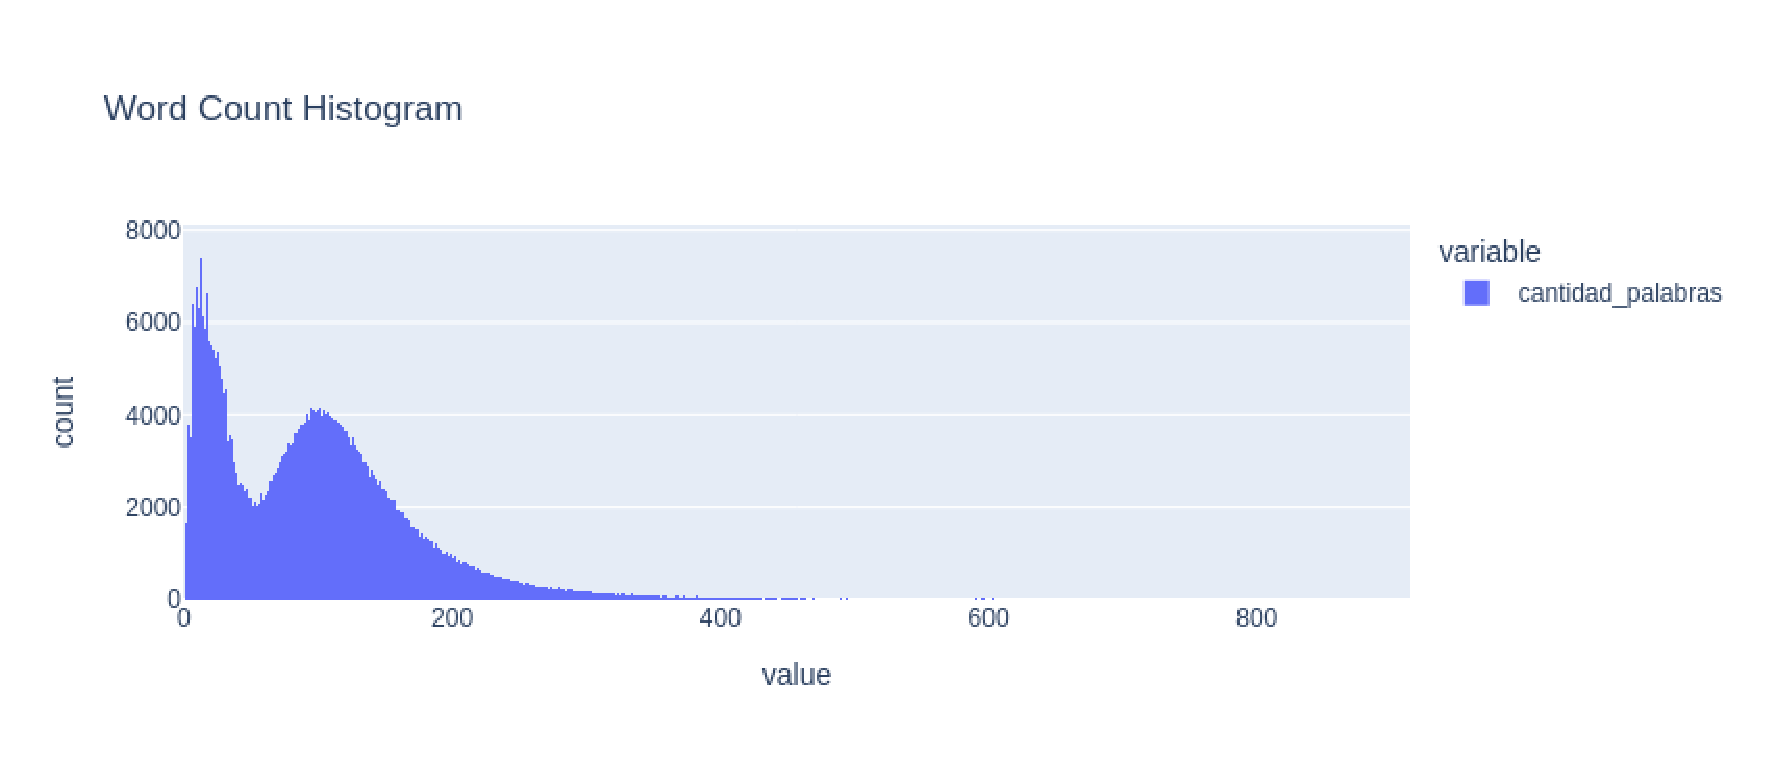
\includegraphics[width=2.5in]{imgs/histograma.eps}
    \caption{Histograma de Cantidad de Palabras $l_w$ en Corpus $D^T$}
    \label{fig:histogramalw}
\end{figure}

\begin{figure}[!t]
    \centering
    \includegraphics[width=2.5in]{imgs/boxplot.png}
    \caption{Diagrama de caja de Cantidad de Palabras $l_w$ en Corpus $D^T$}
    \label{fig:boxplotlw}
\end{figure}

\begin{figure}[!t]
    \centering
    \includegraphics[width=2.5in]{imgs/categorias.png}
    \caption{Categorías de Texto del Dataset $D^T$}
    \label{fig:categorias}
\end{figure}

\begin{table}[!t]
% increase table row spacing, adjust to taste
\renewcommand{\arraystretch}{1.3}
% if using array.sty, it might be a good idea to tweak the value of
% \extrarowheight as needed to properly center the text within the cells
\caption{Valores estadísticos del dataset}
\label{tab: metricasorig}
\centering
% Some packages, such as MDW tools, offer better commands for making tables
% than the plain LaTeX2e tabular which is used here.
\begin{tabular}{c c}
\hline
\textbf{métrica} & \textbf{valor} \\
\hline
cantidad &    \numprint{671146} \\ %count
media     &   \numprint{98.34} \\ %mean
std      &   \numprint{77.38} \\ %std
min      &    \numprint{0} \\ %min
25\%      &   \numprint{33.00} \\
50\%      &   \numprint{92.00} \\
75\%      &  \numprint{137.00} \\
max      &  \numprint{914.00} \\
\hline
\end{tabular}
\end{table}


% Del análisis realizado respecto a la frecuencia de palabras en el texto de la Ndd, se observa que existe un mínimo de $\alpha$y un máximo de $\beta$ palabras. En el diagrama de caja se observa que la media de ejemplos dispone de una cantidad $\eta$ de palabras. De ahí que se seleccionó para la conformación del dataset sólo aquellos ejemplos que disponen de una cantidad de palabras $l_w$ según la Ecuación \ref{eq:limiterelato}

% \begin{equation}\label{eq:limiterelato}
%     \alpha   \leq l_w \leq \beta 
% \end{equation}

\subsubsection{Organización del dataset en subconjuntos de entrenamiento, validación y testeo}

Para realizar el entrenamiento del modelo es necesario separar el dataset $D^T$ en subsets de entrenamiento $D^T_{train}$ (\numprint{273336} registros), validación $D^T_{valid}$ (\numprint{68333} registros) y testeo $D^T_{test}$ (\numprint{90000} registros). Los subsets se obtienen escogiendo ejemplos aleatorios del dataset $D^T$. El dataset de validación se obtuvo separando el dataset de entrenamiento en 80\%, 20\%. De esta manera el entrenamiento del modelo dispone de la cantidad de ejemplos presentada en la Tabla \ref{tab:datasplit}.

\begin{table}[!t]
% increase table row spacing, adjust to taste
\renewcommand{\arraystretch}{1.3}
% if using array.sty, it might be a good idea to tweak the value of
% \extrarowheight as needed to properly center the text within the cells
\caption{Generación de Datasets de Entrenamiento Validación y Testeo}
\label{tab:datasplit}
\centering
% Some packages, such as MDW tools, offer better commands for making tables
% than the plain LaTeX2e tabular which is used here.
\begin{tabular}{ccc}
\hline
Tipo Set & Registros & \%\\
\hline
$D_{train}^T$ & \numprint{273336} & \numprint{63.32}\%\\
$D_{valid}^T$ & \numprint{68333} & \numprint{15.83}\%\\
$D_{test}^T$ & \numprint{90000} & \numprint{20.85}\%\\
\hline
\end{tabular}
\end{table}


Cada dataset está conformado por el texto correspondiente al relato del hecho y una etiqueta numérica que es un número entero desde el 0 al 5, correspondiente a cada una de las etiquetas. Si bien el dataset elaborado dispone de las cantidades mostradas, para esta primera etapa de entrenamiento del modelo se utilizo un subconjunto de datos de cada uno de los datasets debido a las restricciones de hardware para llevar a acabo el entrenamiento del modelo.

%% Poner una tabla de relacion de numero y etiqueta

\subsection{Modelo de Transfer Learning}
Transferlearning, como indica las Ecuaciones \ref{eq:Transfer2} y \ref{eq:Transfer3}, permite ajustar el entrenamiento original $\ypredsource(\cdot)$ adaptándolo a la tarea objetivo $\ypredtarget(\cdot)$. Para esto, se usa una serie de capas representadas por operaciones funcionales $\mathcal{A}$, que permitirán el ajuste del modelo. Durante, el entrenamiento, los pesos del modelo pre-entrenado de \emph{\modelohuggingface} $\ypredsource(\cdot)$, denominados $\mathcal{W}^S$, no son modificados y se usan a modo de \emph{feature extractor} (extractor de características). El modelo pre-entrenado contiene una cantidad de parámetros de $\mathcal{W}^S = \numprint{134734080}$, que no serán entrenados. La salida del modelo pre-entrenado es un tensor $\mathbb{R}^{(N \times 300 \times 768)}$. Usando Global Max Pooling $GMP$, el tensor se transforma a uno de dimensión $\mathbb{R}^{(N \times 768)}$. La aplicación de las operaciones $\mathcal{A}$, descritas en la Ecuación  \ref{eq:finetuning} generan una matriz de pesos $\mathcal{W}^T$ que corresponden a las distintas capas añadidas para este fin. Éstas capas están representadas de manera operacional en la Ecuación \ref{eq:finetuning} y consisten en: Batch Normalization $BN$, Full Connecting Layer con 512 neuronas $FC_{512}$, Drop Out de 0.1 $Dro_{0.1}$, 2 juegos de capas de Full Connecting Layer de 128 $FC_{128}$ y Drop Out de 0.1 $Dro_{0.1}$ y finalmente una capa de salida de 6 neuronas $Fc_{6}$. En consecuencia, no es necesario entrenar la totalidad del modelo final $\mathcal{W}^S+\mathcal{W}^T$, sino únicamente las capas de salida $\mathcal{W}^T$ que corresponde a $\mathcal{W}^T = \numprint{478214}$.

% En el caso de esta investigación, el modelo pre-entrenado  devuelve un vector de 769 componentes luego de aplicar la operación de \emph{max pooling}.  A la salida de este modelo se aplican las siguientes operaciones representadas en manera funcional:

% \begin{align}\label{eq:finetuning}
%     \mathcal{A} = FC_{6} \circ Dro_{0.1} \circ FC_{128}  \circ Dro_{0.1} \circ FC_{128} \circ Dro_{0.1} \\ 
%     \circ FC_{512} \circ BN \circ GMP
% \end{align}

\begin{IEEEeqnarray}{lCr}\label{eq:finetuning}
    \mathcal{A} = FC_{6} \circ Dro_{0.1} \circ FC_{128}  \circ Dro_{0.1} \circ FC_{128} \\ 
    \circ Dro_{0.1} \circ FC_{512} \circ BN \circ GMP \nonumber
\end{IEEEeqnarray}


\subsection{Entrenamiento del modelo}
El entrenamiento del modelo consiste en utilizar \emph{TL} para afinar un modelo pre-entrenado en la tarea de clasificación deseada. De esta manera se podrá predecir la categoría a la que pertenece un texto de robo, escogiendo entre las 6 características antes indicadas (Figura \ref{fig:categorias}). El modelo pre-entrenado utilizado es \emph{\modelohuggingface}. Si bien para obtener el modelo pre-entrenado y la carga del dataset generado se utilizaron las funcionalidades del API de \emph{transformers} de HuggingFace, el entrenamiento del modelo fue realizado en \emph{Tensorflow}. Las etapas para seguidas en el entrenamiento son las siguientes:


% sustituir por gráfico o añadir gráfico
\begin{enumerate}
    \item Carga de los datasets $D^T_{train}$, $D^T_{valid}$, $D^T_{test}$
    \item Tokenización de los datasets
    \item Resampling de los datasets (debido a limitaciones de hardware)
    \item Obtención de los tensores de entrada, máscara y los tensores de clasificación en one-hot encoding.
    \item Carga del modelo pre-entrenado $\ypredsource(\cdot)$
    \item Se obtiene el modelo de ajuste fino aplicando $\mathcal{A}$: $y^T = \ypredtarget(\mathbf{\mathcal{X}}^T) =  \mathcal{A}(\ypredsource(\mathbf{\mathcal{X}}^T))$
    \item Se compila el modelo con los parámetros de entrenamiento presentados en la Tabla \ref{tab:trainingParam}.
    \item Se ejecuta el entrenamiento en Google Colab.
    \item Respaldo de los pesos de entrenamiento.
\end{enumerate}

La tokenización permite convertir el texto a una representación tensorial que es aprovechada por el computador para el entrenamiento del modelo de Machine Learning. Para el caso estudiado, dado que el histograma de la cantidad de palabras por documento indica una secuencia de longitud máxima de $\lambda = 300$ palabras, los tensores de máscara y entrada son de $\mathbf{\mathcal{X}}^{N\times300}$;donde $N$ es la cantidad de ejemplos.

Debido a las limitaciones en el hardware utilizado para el entrenamiento (Google Colab), los ejemplos reducidos a $d^T_{train}:\numprint{20000} \subset D^T_{train}$, $d^T_{valid}:\numprint{4000} \subset D^T_{valid}$, $d^T_{test}:\numprint{4000} \subset D^T_{test}$.

\begin{table}[!t]
% increase table row spacing, adjust to taste
\renewcommand{\arraystretch}{1.3}
% if using array.sty, it might be a good idea to tweak the value of
% \extrarowheight as needed to properly center the text within the cells
\caption{Parámetros de Entrenamiento}
\label{tab:trainingParam}
\centering
% Some packages, such as MDW tools, offer better commands for making tables
% than the plain LaTeX2e tabular which is used here.
\begin{tabular}{cc}
\hline
Parámetro & Valor\\
\hline
 Loss & Categorical Cross Entropy\\
Metrics & Categorical Accuracy \\
Optimizer & Adam \\
Learning rate & $2 \times 10^{-4}$ \\
epochs & 10 \\
callback & 5 epochs \\
\hline
\end{tabular}
\end{table}

\section{Resultados Experimentales}\label{chap:resultados}
Los resultados del entrenamiento se muestran en la Figura \ref{fig:loss80} y \ref{fig:train80} para la función de optimización y la métrica de rendimiento respectivamente. El modelo ajustado obtuvo un \emph{accuracy} de \numprint{0.8248}, en el dataset de entrenamiento, \numprint{0.8048}, en el dataset de validación y \numprint{0.8045} para el dataset de prueba. 


\begin{figure*}[!t]
\centering
\subfloat[Loss]{\includegraphics[width=2.5in]{imgs/losstrainacc80.png}
\label{fig:loss80}}
\hfil
\subfloat[Accuracy]{\includegraphics[width=2.5in]{imgs/trainacc80.png}
\label{fig:train80}}
\caption{Entrenamiento del Modelo de Machine Learning Clasificación de Texto}
\label{fig: results}
\end{figure*}

En cuanto a la métrica de $f_1score$ se obtuvo en promedio 0.80; en donde el resultado más bajo se obtiene para la clase 0 con un valor de 0.45 y el más alto de 0.87 en la clase 1. Los resultados del clasificador sobre el dataset de pruebas se presentan en la Tabla \ref{tab:fscore}, donde se observa el rendimiento del recall y el f-score.


\begin{table}[!t]
% increase table row spacing, adjust to taste
\renewcommand{\arraystretch}{1.3}
% if using array.sty, it might be a good idea to tweak the value of
% \extrarowheight as needed to properly center the text within the cells
\caption{Rendimiento del clasificador}
\label{tab:fscore}
\centering
% Some packages, such as MDW tools, offer better commands for making tables
% than the plain LaTeX2e tabular which is used here.
\begin{tabular}{ccccc}

\hline
         class &  precision  &  recall & f1-score &  support \\ \hline

           0 &  \numprint{0.58}    &  \numprint{0.36}    &  \numprint{0.45}  &  \numprint{285} \\ 
           1 &   \numprint{0.90}    &  \numprint{0.84}    &  \numprint{0.87}  &  \numprint{457} \\
           2 &   \numprint{0.79}    &  \numprint{0.79}    &  \numprint{0.79}  &  \numprint{613} \\
           3 &   \numprint{0.82}    &  \numprint{0.91}    &  \numprint{0.86}  & \numprint{1666} \\
           4 &   \numprint{0.82}    &  \numprint{0.70}    &  \numprint{0.75}  &  \numprint{328} \\
           5 &   \numprint{0.76}    &  \numprint{0.77}    &  \numprint{0.77}  &  \numprint{651} \\ \hline

   micro avg &     \numprint{0.80} &    \numprint{0.80}   &  \numprint{0.80}  &   \numprint{4000} \\ 
   macro avg &     \numprint{0.78} &    \numprint{0.73}   &  \numprint{0.75}  &   \numprint{4000} \\ \hline
% weighted avg       0.80      0.80      0.80      4000
%  samples avg       0.80      0.80      0.80      4000

\hline
\end{tabular}
\end{table}


 
 
% An example of a floating figure using the graphicx package.
% Note that \label must occur AFTER (or within) \caption.
% For figures, \caption should occur after the \includegraphics.
% Note that IEEEtran v1.7 and later has special internal code that
% is designed to preserve the operation of \label within \caption
% even when the captionsoff option is in effect. However, because
% of issues like this, it may be the safest practice to put all your
% \label just after \caption rather than within \caption{}.
%
% Reminder: the "draftcls" or "draftclsnofoot", not "draft", class
% option should be used if it is desired that the figures are to be
% displayed while in draft mode.
%
%\begin{figure}[!t]
%\centering
%\includegraphics[width=2.5in]{myfigure}
% where an .eps filename suffix will be assumed under latex, 
% and a .pdf suffix will be assumed for pdflatex; or what has been declared
% via \DeclareGraphicsExtensions.
%\caption{Simulation results for the network.}
%\label{fig_sim}
%\end{figure}

% Note that the IEEE typically puts floats only at the top, even when this
% results in a large percentage of a column being occupied by floats.


% An example of a double column floating figure using two subfigures.
% (The subfig.sty package must be loaded for this to work.)
% The subfigure \label commands are set within each subfloat command,
% and the \label for the overall figure must come after \caption.
% \hfil is used as a separator to get equal spacing.
% Watch out that the combined width of all the subfigures on a 
% line do not exceed the text width or a line break will occur.
%
%\begin{figure*}[!t]
%\centering
%\subfloat[Case I]{\includegraphics[width=2.5in]{box}%
%\label{fig_first_case}}
%\hfil
%\subfloat[Case II]{\includegraphics[width=2.5in]{box}%
%\label{fig_second_case}}
%\caption{Simulation results for the network.}
%\label{fig_sim}
%\end{figure*}
%
% Note that often IEEE papers with subfigures do not employ subfigure
% captions (using the optional argument to \subfloat[]), but instead will
% reference/describe all of them (a), (b), etc., within the main caption.
% Be aware that for subfig.sty to generate the (a), (b), etc., subfigure
% labels, the optional argument to \subfloat must be present. If a
% subcaption is not desired, just leave its contents blank,
% e.g., \subfloat[].


% An example of a floating table. Note that, for IEEE style tables, the
% \caption command should come BEFORE the table and, given that table
% captions serve much like titles, are usually capitalized except for words
% such as a, an, and, as, at, but, by, for, in, nor, of, on, or, the, to
% and up, which are usually not capitalized unless they are the first or
% last word of the caption. Table text will default to \footnotesize as
% the IEEE normally uses this smaller font for tables.
% The \label must come after \caption as always.
%
%\begin{table}[!t]
%% increase table row spacing, adjust to taste
%\renewcommand{\arraystretch}{1.3}
% if using array.sty, it might be a good idea to tweak the value of
% \extrarowheight as needed to properly center the text within the cells
%\caption{An Example of a Table}
%\label{table_example}
%\centering
%% Some packages, such as MDW tools, offer better commands for making tables
%% than the plain LaTeX2e tabular which is used here.
%\begin{tabular}{|c||c|}
%\hline
%One & Two\\
%\hline
%Three & Four\\
%\hline
%\end{tabular}
%\end{table}


% Note that the IEEE does not put floats in the very first column
% - or typically anywhere on the first page for that matter. Also,
% in-text middle ("here") positioning is typically not used, but it
% is allowed and encouraged for Computer Society conferences (but
% not Computer Society journals). Most IEEE journals/conferences use
% top floats exclusively. 
% Note that, LaTeX2e, unlike IEEE journals/conferences, places
% footnotes above bottom floats. This can be corrected via the
% \fnbelowfloat command of the stfloats package.




\section{Conclusiones}\label{chap:conclusion}
Los modelos basados en \emph{Transformers} han obtenido un desempeño mejorado en los problemas de procesamiento de lenguaje natural; siendo hoy por hoy el estado del arte. En este artículo se ha realizado el ajuste fino de un modelo pre-entrenado para la clasificación de relatos de robos en 6 categorías. 

Los resultados muestran que a pesar de que el dataset no tiene un balance de los ejemplos de cada clase (siendo la clase Robo a Personas la que más ejemplos dispone), la utilización de \emph{TL} desde el modelo pre-entrenado de \modelohuggingface\, permite obtener un rendimiento muy bueno para iniciar las pruebas piloto en la predicción de nuevos casos. Los resultados en f-score también indican que a excepción del bajo performance en la clase 0, se obtiene en promedio un rendimiento del 80\%.

Como resultado de la investigación se concluye que el campo de las leyes es muy propicio para el desarrollo de modelos de inteligencia artificial, que apoyados en el estado del arte, pueden generar nuevos servicios, automatizar tareas, y mejorar la calidad del trabajo realizado en instituciones de importancia estratégica como la Fiscalía General del Estado.


\section{Trabajos Futuros}\label{chap:futuro}

Como trabajo futuro se plantea realizar el entrenamiento del modelo en dos escenarios: 

\begin{enumerate}
    \item Entrenamiento con subconjunto de datos $d^T$ con balanceo de registros por clase.
    \item Entrenamiento con el conjunto total de datos $D^T$ sin balanceo de clases.
    \item Entrenamiento con el conjunto total de datos $D^T$ con balanceo de clases.
\end{enumerate}

Adicionalmente se iniciará una etapa de pruebas del modelo actualmente entrenados que serán contrastadas con la clasificación manual realizada en la Comisión.


% if have a single appendix:
%\appendix[Proof of the Zonklar Equations]
% or
%\appendix  % for no appendix heading
% do not use \section anymore after \appendix, only \section*
% is possibly needed

% use appendices with more than one appendix
% then use \section to start each appendix
% you must declare a \section before using any
% \subsection or using \label (\appendices by itself
% starts a section numbered zero.)
%


% \appendices
% \section{Proof of the First Zonklar Equation}
% Appendix one text goes here.

% you can choose not to have a title for an appendix
% if you want by leaving the argument blank
% \section{}
% Appendix two text goes here.


% use section* for acknowledgment
\section*{Agradecimientos}


% The authors would like to thank...
Los autores desean agradecer a la Fiscalía General del Estado por permitir realizar investigación en la realización de modelos de \emph{machine learning} en problemas de procesamiento de lenguaje natural aplicados a tareas propias de la institución. Se agradece el apoyo de la Dirección de Estadística y Sistemas de información que generó el dataset para la investigación realizada. 


% Can use something like this to put references on a page
% by themselves when using endfloat and the captionsoff option.
\ifCLASSOPTIONcaptionsoff
  \newpage
\fi



% trigger a \newpage just before the given reference
% number - used to balance the columns on the last page
% adjust value as needed - may need to be readjusted if
% the document is modified later
%\IEEEtriggeratref{8}
% The "triggered" command can be changed if desired:
%\IEEEtriggercmd{\enlargethispage{-5in}}

% references section

% can use a bibliography generated by BibTeX as a .bbl file
% BibTeX documentation can be easily obtained at:
% http://mirror.ctan.org/biblio/bibtex/contrib/doc/
% The IEEEtran BibTeX style support page is at:
% http://www.michaelshell.org/tex/ieeetran/bibtex/
%\bibliographystyle{IEEEtran}
% argument is your BibTeX string definitions and bibliography database(s)
%\bibliography{IEEEabrv,../bib/paper}
%
% <OR> manually copy in the resultant .bbl file
% set second argument of \begin to the number of references
% (used to reserve space for the reference number labels box)

% \begin{thebibliography}{1}

% \bibitem{IEEEhowto:kopka}
% H.~Kopka and P.~W. Daly, \emph{A Guide to \LaTeX}, 3rd~ed.\hskip 1em plus
%   0.5em minus 0.4em\relax Harlow, England: Addison-Wesley, 1999.

% \end{thebibliography}

% \bibliography{./bibtex/mybib.bib}
\printbibliography

% biography section
% 
% If you have an EPS/PDF photo (graphicx package needed) extra braces are
% needed around the contents of the optional argument to biography to prevent
% the LaTeX parser from getting confused when it sees the complicated
% \includegraphics command within an optional argument. (You could create
% your own custom macro containing the \includegraphics command to make things
% simpler here.)
%\begin{IEEEbiography}[{\includegraphics[width=1in,height=1.25in,clip,keepaspectratio]{mshell}}]{Michael Shell}
% or if you just want to reserve a space for a photo:

% ======== bibiografía =============
% \begin{IEEEbiography}{Michael Shell}
% Biography text here.
% \end{IEEEbiography}

% % if you will not have a photo at all:
% \begin{IEEEbiographynophoto}{John Doe}
% Biography text here.
% \end{IEEEbiographynophoto}

% % insert where needed to balance the two columns on the last page with
% % biographies
% %\newpage

% \begin{IEEEbiographynophoto}{Jane Doe}
% Biography text here.
% \end{IEEEbiographynophoto}

% You can push biographies down or up by placing
% a \vfill before or after them. The appropriate
% use of \vfill depends on what kind of text is
% on the last page and whether or not the columns
% are being equalized.

%\vfill

% Can be used to pull up biographies so that the bottom of the last one
% is flush with the other column.
%\enlargethispage{-5in}



% that's all folks
\end{document}





%%% Local Variables:
%%% mode: LaTeX
%%% TeX-master: t
%%% End:
